\documentclass[12pt]{article}
\usepackage[english]{babel}
\usepackage[utf8x]{inputenc}
\usepackage[T1]{fontenc}
\usepackage{scribe}
\usepackage{listings}
\usepackage{tikz}

\Scribe{\small{Group 13, Group 14}}
\Lecturer{Abir De}
\LectureNumber{7}
\LectureDate{August $29^{th},2022$}
\LectureTitle{Linear Regression- Regularization and Stability}

\lstset{style=mystyle}

\begin{document}
	\MakeScribeTop

%#############################################################
%#############################################################
%#############################################################
%#############################################################

\noindent In the previous lecture, we briefly discussed the regression problem and explained the different types of loss functions we can use to train a regression model. This lecture will be a continuation of the linear regression problem and we will introduce a very important technique to improve loss functions called regularization. In the later part of this lecture, we will learn about a new feature of models called "stability". 

\section{Choosing between loss functions: MSE vs Absolute Error}

In the previous class, we also discussed the comparison between MSE loss function and the absolute error function. We had discussed that minimizing the MSE loss is akin to obtaining the maximum likelihood estimate for the target function $f$, assuming that the noise in the $y$ was sampled from a Gaussian distribution. 


Similarly, minimizing the absolute error loss is the same as obtaining the MLE for the target function given that the noise was sampled from a Laplacian Distribution. 

The user prefers the absolute error function when the user wants to maximize the number of correct predictions, but does not care much about the error when a prediction is wrong. On the other hand, the MSE loss function is preferred when the difference between the actual value and the predicted value is also of significance.

\section{Regression}

Continuing where we left in the last class, we have the following loss function which needs to be minimized to get optimal parameters for the regression problem:

\begin{gather}
    L(\boldsymbol{w},b) = \sum_{i \in D}   (y_i - \boldsymbol{w}^T\boldsymbol{x_i} - b)^2              \nonumber\\
    \begin{aligned}
        \text{s.t.} \quad   y_i \in \mathbb{R},  \quad \boldsymbol{x_i} \in \mathbb{R}^d \quad i.e. \quad \boldsymbol{x_i} = \begin{bmatrix} x_i^1 & x_i^2 & \cdots & x_i^d\end{bmatrix}^T
        \nonumber\\
    \end{aligned}
\end{gather}\\
Here, dataset $D = \{\boldsymbol{x_i},y_i\}$ is the set of all points over which the analysis is done, $\boldsymbol{x_i}$ is the input vector for $i^{th}$ sample and $d$ is the number of features in each vector $\boldsymbol{x_i}$. $y_i$ is the \textbf{label} associated with each \textbf{sample} $\boldsymbol{x_i}$ and \textbf{weight} $\boldsymbol{w} \in \mathbb{R}^d$ is the vector of weights assigned to each individual feature. \\
\\
%%%%%%%%%%%%%%%%%%%%%%%%%%%%%%%%%%%%%%%%%%%%%%%%
%%%%%%%%%%%%%%%%%%%%%%%%%%%%%%%%%%%%%%%%%%%%%%%%
%%%%%%%%%%%%%%%%%%%%%%%%%%%%%%%%%%%%%%%%%%%%%%%%
%%keeping on hold till dimensions clarified
Observe that we can avoid explicitly mentioning $b$ in the loss function, since it is a scalar and a modification of $\boldsymbol{x_i}$ can incorporate it. Thus our minimization problem reduces to:

\begin{gather}
    \begin{aligned}
        \min_{\boldsymbol{w}} L'(\boldsymbol{w}) & = \quad \min_{\boldsymbol{w}} \quad \sum_{i \in D}   (y_i - \boldsymbol{w}^T\boldsymbol{x_i})^2              \nonumber\\
        & = \quad \min_{\boldsymbol{w}} \quad \sum_{i \in D}   (y_i^2 - 2\boldsymbol{w}^T\boldsymbol{x_i}y_i + (\boldsymbol{w}^T\boldsymbol{x_i})^2)\nonumber\\
        & = \quad \min_{\boldsymbol{w}} \quad (\vec{\boldsymbol{y}}-\boldsymbol{X}\boldsymbol{w})^T(\vec{\boldsymbol{y}}-\boldsymbol{X}\boldsymbol{w})\nonumber\\
        & = \quad \min_{\boldsymbol{w}} \quad (\vec{\boldsymbol{y}}^T\vec{\boldsymbol{y}}- 2\vec{\boldsymbol{y}}^T\boldsymbol{X}\boldsymbol{w} + \boldsymbol{w}^T\boldsymbol{X}^T\boldsymbol{X}\boldsymbol{w}) \nonumber \\
    \end{aligned}
\end{gather}

\begin{gather}
    \begin{aligned}
        & \text{where}  \quad \vec{\boldsymbol{y}} = \begin{bmatrix} y_1 \\ y_2 \\ \vdots \\ y_n\end{bmatrix} , \quad \boldsymbol{X} = \begin{bmatrix} \boldsymbol{x_1}^T \\ \boldsymbol{x_2}^T \\ \vdots \\ \boldsymbol{x_n}^T\end{bmatrix} \text{and} \quad n = |D| \nonumber
    \end{aligned}
\end{gather}

\noindent On differentiating w.r.t $\boldsymbol{w}$ and equating the \textit{gradient} to 0, we get:
\begin{gather}
    \begin{aligned}
        \nabla_{\boldsymbol{w}}L'(\boldsymbol{w}) = 2\boldsymbol{X}^T(\boldsymbol{X}\boldsymbol{w} - \vec{\boldsymbol{y}}) &= 0 \nonumber \\
        \quad \boldsymbol{X}^T\vec{\boldsymbol{y}} &= \boldsymbol{X}^T\boldsymbol{X}\boldsymbol{w}            \nonumber\\
        \quad \boldsymbol{w} &= (\boldsymbol{X}^T\boldsymbol{X})^{-1}\boldsymbol{X}^T\vec{\boldsymbol{y}}  \nonumber\\
        \quad \boldsymbol{w} &= (\boldsymbol{X}^T\boldsymbol{X})^{-1}\sum_{i \in D}y_i\boldsymbol{x_i}
    \end{aligned}
\end{gather}
%%%%%%%%%%%%%%%%%%%%%%%%%%%%%%%%%%%%%%%%%%%%%%%
%%%%%%%%%%%%%%%%%%%%%%%%%%%%%%%%%%%%%%%%%%%%%%%
%%%%%%%%%%%%%%%%%%%%%%%%%%%%%%%%%%%%%%%%%%%%%%%
% Here's a citation~\cite{Kar84a}.
\\
Thus, we have an expression for the optimal $\boldsymbol{w}$ ($\boldsymbol{w}^*$). Observe: we need $\boldsymbol{X}^T\boldsymbol{X}$ to be invertible for this model to work. In the following subsection, we will discuss this in detail.

\subsection{Invertibility of $\boldsymbol{X}^T\boldsymbol{X}$}
Note that, $\boldsymbol{X}^T\boldsymbol{X}$ will be invertible if and only if the determinant of the matrix $\boldsymbol{X}^T\boldsymbol{X}$ is non-zero, $i.e.$, the matrix is non singular.\\ \\
We know that each $\boldsymbol{x_i}$ is an i.i.d (identical, independent draw) from a continuous distribution. Thus for $n > d$ where $\boldsymbol{X}$ is of dimensions $n \times d$, we can claim that $|\boldsymbol{X}^T\boldsymbol{X}|$ has a continuous distribution. Hence, the probability that determinant of $\boldsymbol{X}^T\boldsymbol{X}$ will take exactly 0 value is 0, $i.e.$ 
\begin{gather}
    \begin{aligned}
        &  P(|\boldsymbol{X}^T\boldsymbol{X}| = 0) = 0           \nonumber
    \end{aligned}
\end{gather}
Intuitively, we can also see that the matrix $X$ is highly likely to be full rank. A $dxN$ matrix (where $N \ge d$) is full rank if atleast $d$ columns out of the $N$ columns are linearly independent.
% Since the function $|\boldsymbol{X}^T\boldsymbol{X}|$ will become 0 at discrete points thus, net probability for $|\boldsymbol{X}^T\boldsymbol{X}| = 0$ is zero. \\
% \\ 
At the same time, note that the probability of $|\boldsymbol{X}^T\boldsymbol{X}|$ lying within some $\epsilon$ near 0 is not zero $i.e.$ $P(|\boldsymbol{X}^T\boldsymbol{X}| < \epsilon) \neq 0$ 

In mathematics, a condition number is a number representative of the change of an output proportionate to a change in the input of a function. For example, if a small change in the input results in a small change in the output, the function produces a small condition number and is said to be well-conditioned. Alternatively, if a small change in the input results in a large change in the output, the function produces a large condition number and is defined as ill-conditioned. The condition number is mathematically given as the ratio of the maximum and minimum eigenvalues. 

Poorly conditioned matrix A is a matrix with a high condition number. $A^{-1}$ amplifies input errors. Small errors in x can change the output of $A^{-1}x$ rapidly. 

\begin{definition}
Condition number of a matrix A is the ratio of its minimum eigenvalue to maximum eigenvalue
\begin{gather}
    \begin{aligned}
        &  Cond(\boldsymbol{A})= \frac{min(eigen(\boldsymbol{A}))}{max(eigen(\boldsymbol{A}))}           \nonumber\\
    \end{aligned}
\end{gather}
\end{definition}
%explain $n>d$, condition num dependence for invertibility\\
%Condition number measures how much the output can change for a small change in the input data or any roundoff errors.

\noindent Condition number of a matrix \textbf{A} is a good indicator of the invertibility of the matrix. A high condition number results in a well conditioned matrix which increases the chances of \textbf{A} being invertible, whereas, a low condition number results in an ill conditioned matrix, $i.e.$ reduced chances of invertiblilty.
\\
\\
We want to ensure that the matrix $\boldsymbol{X}^T\boldsymbol{X}$ is well-conditioned. One possible approach for this is replacing $\boldsymbol{X}^T\boldsymbol{X}$ with $ \boldsymbol{X}^T\boldsymbol{X} + \lambda\boldsymbol{I}$, $i.e.$
\begin{gather}
    \begin{aligned}
        &  \boldsymbol{w}* = (\boldsymbol{X}^T\boldsymbol{X} + \lambda\boldsymbol{I})^{-1}\boldsymbol{X}^T\vec{\boldsymbol{y}}      \nonumber\\
    \end{aligned}
\end{gather}
Note here that such a transformation changes the condition number as follows:
\begin{gather}
    \begin{aligned}
        & Cond(\boldsymbol{X}^T\boldsymbol{X}) \to Cond(\boldsymbol{X}^T\boldsymbol{X} + \lambda\boldsymbol{I})    \nonumber\\
        & \frac{min(eigen(\boldsymbol{X}^T\boldsymbol{X}))}{max(eigen(\boldsymbol{X}^T\boldsymbol{X}))} \to \frac{min(eigen(\boldsymbol{X}^T\boldsymbol{X} + \lambda\boldsymbol{I}))}{max(eigen(\boldsymbol{X}^T\boldsymbol{X}+ \lambda\boldsymbol{I}))}  \nonumber \\
        & \frac{a}{b} \to \frac{a+\lambda}{b+\lambda} \quad (\text{assuming} \quad Cond(\boldsymbol{X}^T\boldsymbol{X}) = \frac{a}{b}) \nonumber \\
    \end{aligned}
\end{gather}
Thus, the $\lambda\boldsymbol{I}$ term adds a lower bound to the value of condition number improving the chances of invertibility of desired matrix.\\
\\
\noindent Also, we find that this type of $\boldsymbol{w}*$ is the solution to the following loss minimization problem:
\begin{gather}
    \begin{aligned}
        & \min_{\boldsymbol{w}} \quad \sum_{i \in D}   (y_i - \boldsymbol{w}^T\boldsymbol{x_i})^2  + \lambda\|\boldsymbol{w}\|^2           \nonumber\\
    \end{aligned}
\end{gather}
More about this in the next section.

\section{Regularization}

Theoretically, \textbf{regularization} is a popular technique used to reduce errors by fitting the function appropriately on the given training set and to avoid overfitting \\
% Overfitting occurs when the model is constraint to the training set and not able to perform well on the test set, here the gap between the training error and testing error is too large\\
\\ The most common regularization techniques are:
\begin{enumerate}
    \item L1 regularization
    \item L2 regularization
    \item Dropout regularization
\end{enumerate}

\noindent Here we will discuss L2 regularization.\\
\\
We saw an example of L2 regularization at the end of the last section trying to ensure that the matrix whose inverse we are calculating is well conditioned. Following was the loss minimization expression for it:
\begin{gather}
    \begin{aligned}
        & \min_{\boldsymbol{w}} \quad \sum_{i \in D}   (y_i - \boldsymbol{w}^T\boldsymbol{x_i})^2  + \lambda\|\boldsymbol{w}\|^2           \nonumber\\
    \end{aligned}
\end{gather}
%%%%%%%%%%%%%%%%%%%%%%%%%%%%%%%%%%%%%%%%%%%%%%%%
%%%%%%%%%%%%%%%%%%%%%%%%%%%%%%%%%%%%%%%%%%%%%%%%
%%%%%%%%%%%%%%%%%%%%%%%%%%%%%%%%%%%%%%%%%%%%%%%%
%%keeping on hold till dimensions clarified
Here, $\lambda\|\boldsymbol{w}\|^2$ is called the \textbf{regularizer} term. In the following sections, we discuss some \textbf{advantages} of regularization.
\subsection{Ensures Well-Conditioned Matrix}

As we saw in \textbf{Section 1.1}, if we add the L2 regularizer term to our Loss function then the solution for the optimal $\boldsymbol{w}^*$ will be:
\begin{gather}
    \begin{aligned}
        &  \boldsymbol{w}* = (\boldsymbol{X}^T\boldsymbol{X} + \lambda\boldsymbol{I})^{-1}\boldsymbol{X}^T\vec{\boldsymbol{y}}      \nonumber\\
    \end{aligned}
\end{gather}
Instead of:
\begin{gather}
    \begin{aligned}
        &  \boldsymbol{w}* = (\boldsymbol{X}^T\boldsymbol{X})^{-1}\boldsymbol{X}^T\vec{\boldsymbol{y}}      \nonumber\\
    \end{aligned}
\end{gather}
\\
The regularizer adds a lower bound to the condition number of the desired matrix matrix, thus increasing the chances of invertibility of $\boldsymbol{X}^T\boldsymbol{X} + \lambda\boldsymbol{I}$ compared to $\boldsymbol{X}^T\boldsymbol{X}$.
\subsection{Prevents Overfitting}
\textbf{Overfitting} occurs when the model is constrained to the training set and not able to perform well on the test set, here the gap between the training error and testing error is large. \\\\
\textbf{Example:}\\
Let us look at a regularization problem with the following loss function:\\
\begin{gather}
    \begin{aligned}
        & \min_{\boldsymbol{w}} \quad \sum_{i \in D}   (y_i - \boldsymbol{w}^T\boldsymbol{x_i})^2            \nonumber\\
    \end{aligned}
\end{gather}
\\
Suppose the number of features in each data point $\boldsymbol{x_i}$ in the dataset increases significantly say from $d_1$ to $d_2$ such that $d_2 > d_1$. In response to this, the dimensions of our learnable parameter $\boldsymbol{w}$ also change from $d_1\times 1$ to $d_2\times 1$ . Thus, the overall model will become more \textbf{complicated}. \\
Also, more features will help bring down the training loss and will increase the training accuracy, but since the model has been trained on the same training set with more features, it loses \textbf{generalization}. The \textbf{test accuracy} will become significantly \textbf{low}er due to this overfitting of model on training data.  
\subsubsection{How to avoid overfitting?}
The solution is again regularization. On adding regularizer term to our original L2-loss, we obtain the new loss function as follows:
\begin{gather}
    \begin{aligned}
        & \min_{\boldsymbol{w}} \quad \sum_{i \in D}   (y_i - \boldsymbol{w}^T\boldsymbol{x_i})^2  + \lambda\|\boldsymbol{w}\|^2           \nonumber\\
    \end{aligned}
\end{gather}
\\
If the number of features of $\boldsymbol{x_i}$ increases then the dimension of $\boldsymbol{w}$ will also increase, and hence the dimension of $\boldsymbol{w}*$ will increase. Due to this increase in dimension the value of the  regularizer term $\lambda\|\boldsymbol{w}\|^2$ rises, increasing the overall loss value. \\
\\
So, the training loss can be greater with a higher number of features compared to one obtained with less number of features $i.e.$ with the regularized loss function, a model with higher number of features is not necessarily a better model for the training set. This helps prevent overfitting of the model.

\subsubsection{Alternate technique to avoid overfitting}
If regularization is not allowed, how to decide the optimal number of features to train the model?\\
\\We can use the method discussed here to find the optimal subset of features to be used for a training set with a large number of extractable information/features. Let the total number of features be $d$, the algorithm follows below:
\begin{itemize}
    \item Separate a portion of the training data as \textbf{validation set}.
    \item Iterate over all subsets $\boldsymbol{s}$ of features with cardinality  $|\boldsymbol{s}| = d' \leq d$
    \item Compare across all these subsets by finding their loss on the validation set. Choose the set of features that gives minimum loss on the validation set.  
\end{itemize}
The above steps can be summarized by the following loss function:
\begin{gather}
    \begin{aligned}
        & \min_{\boldsymbol{w_s,s}} \quad \sum_{i \in D}   (y_i - \boldsymbol{w}^T_s\boldsymbol{x_{i,s}})^2          \nonumber\\
    \end{aligned}
\end{gather}
\noindent Here, $|\boldsymbol{s}|\leq d$  and $\boldsymbol{x_{i,s}}$ refers to the subset of $\boldsymbol{x_i}$ which has features corresponding to the set $\boldsymbol{s}$.
\\ \\
But this optimization problem is \textbf{NP Hard} due to the exponential search space involving iteration over all subsets. 
\section{Stability}
A model is called stable if on addition of a new data point to training dataset, the learnable parameter $\boldsymbol{w}$ does not change very much. 
\\ \\
Mathematically speaking, let $D$ be our initial training dataset and $D \cup k$ be the new training dataset with the addition of a new data point $k$. Then we define the following quantity:   
\begin{gather}
    \begin{aligned}
        & l = \|\boldsymbol{w}^*_{(D)} - \boldsymbol{w}^*_{(D \cup k)}\| \nonumber
    \end{aligned}
\end{gather}
Stability is ensured when this $l$ is small. This means that on addition/modification/removal of a data point, the learnable parameter $\boldsymbol{w}$ did not $change$ very much.\\
\\
Mathematically, we call a model stable if $l$ follows this condition:
\begin{gather}
    \begin{aligned}
        & l = \|\boldsymbol{w}^*_{(D)} - \boldsymbol{w}^*_{(D \cup k)}\| < \epsilon, \quad \text{where} \quad \epsilon \sim O(\frac{1}{n}) = O({\frac{1}{|D|}}) \nonumber
    \end{aligned}
\end{gather}
where $|D|$ = $n$  is the size of the complete dataset.
\\ \\
We can prove that if the model follows the stability condition stated above then, $$\text{test-case error} \leq \alpha\epsilon + \beta$$
where, $\alpha$ and $\beta$ are constants that are not in our control but $\epsilon$ is decided by model predictions. 
\\ \\The constant $\beta$ is decided by the quality of dataset provided. For example if, $\boldsymbol{x_i}$ is sampled from a normal distribution $\mathcal{N}(0,1)$ and corresponding $y_i$ are sampled from  uniform distribution $U(0,1)$, then the value of constant $\beta$ will be higher since dataset is randomly created.
\subsection{Advantages of Stability}
\subsubsection{Smaller dataset needed for training}
    When a model is trained on a small dataset $D$ but is stable, then on addition of a new data point \textbf{k} the optimal learnable parameter $\boldsymbol{w*}$ does not change a lot $i.e.$, the previously learned $w^*(D)$ is similar to $w^*(D \cup k)$ even on addition of a new unseen point. \\
    \\
    Thus, our model behaves as if it has been trained on the larger set and will also work well on unseen test samples.    
\subsubsection{Prevents leak of information to adversary}
    This is one of the information security concerns of the model. Suppose on addition of a data point $k$, the model's learnable parameter $\boldsymbol{w}^*$ changes a lot. This can reveal important characteristics of the model to the adversary which can be used to predict label $y_i$ of the model on input $x_i$ with some confidence and thus an adversary can exploit the model.
    \\
    \\ To understand this point better, let us present a small example:\\
    \\
    Suppose A, B, C, D are 4 people on Facebook. As shown in the diagram below, Person A has a private Facebook connection with D which is not visible to others. All other connections are publicly visible. \\
    \begin{center}
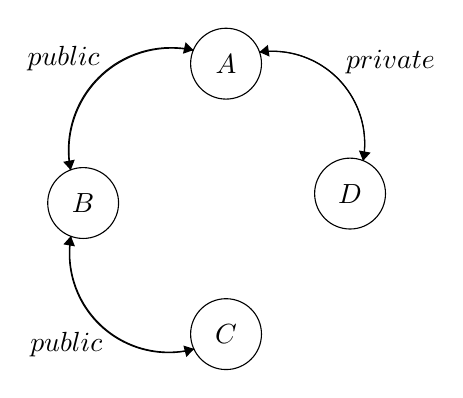
\begin{tikzpicture}[scale=0.15]
\tikzstyle{every node}+=[inner sep=0pt]
\draw [black] (38.4,-13.4) circle (3);
\draw (38.4,-13.4) node {$A$};
\draw [black] (38.4,-36.3) circle (3);
\draw (38.4,-36.3) node {$C$};
\draw [black] (48.9,-24.4) circle (3);
\draw (48.9,-24.4) node {$D$};
\draw [black] (26.3,-25.2) circle (3);
\draw (26.3,-25.2) node {$B$};
\draw [black] (41.217,-12.422) arc (98.15737:-10.82181:7.821);
\fill [black] (41.22,-12.42) -- (42.08,-12.8) -- (41.94,-11.81);
\draw (48.51,-13.29) node [right] {$private$};
\draw [black] (41.22,-12.432) arc (97.96314:-10.62758:7.828);
\fill [black] (50,-21.63) -- (50.64,-20.93) -- (49.65,-20.75);
\draw [black] (35.692,-37.554) arc (-75.37126:-189.6925:8.406);
\fill [black] (35.69,-37.55) -- (34.79,-37.27) -- (35.04,-38.24);
\draw (24.87,-36.1) node [below] {$public$};
\draw [black] (25.22,-22.417) arc (-168.69679:-282.74152:8.679);
\fill [black] (35.65,-12.25) -- (34.97,-11.59) -- (34.75,-12.56);
\draw (24.65,-14.02) node [above] {$public$};
\draw [black] (25.25,-22.406) arc (-169.27384:-282.16447:8.702);
\fill [black] (25.25,-22.41) -- (25.59,-21.53) -- (24.61,-21.71);
\draw [black] (35.703,-37.578) arc (-74.88975:-190.17401:8.389);
\fill [black] (25.26,-28) -- (24.63,-28.7) -- (25.61,-28.87);
\end{tikzpicture}
\end{center}
    Now suppose that the Facebook algorithm recommends Person D's profile to Person C, then C can estimate with certain confidence that either of B or A has a private connection with D. If Person C get to know that Person B has no private connection then Person C can say with certainty that Person A has a private connection with Person D. \\
    \\
    Thus, the recommendation algorithm of Facebook's model could have been designed better to ensure data privacy in such a case.

\subsection{Individual and Overall Loss}
\begin{definition}
Individual loss: $l(\boldsymbol{w}^T\boldsymbol{x_i},y_i) = (y_i - \boldsymbol{w}^T\boldsymbol{x_i})^2 + \lambda \|\boldsymbol{w}\|^2$
\end{definition}
\begin{definition}
Overall loss: $\sum_{i\in D} l(\boldsymbol{w}^T\boldsymbol{x_i},y_i) $ 
\end{definition}
\noindent Notice the subtle difference between the regularized l2-loss introduced in section 2 and the overall loss function described here. In the overall loss definition, $\lambda\|w\|^2$ will be repeated $|D|$ times where $|D|$ is the size of the dataset while in the regularized l2-loss, it is included exactly once.\\
\\
The relation between $\lambda$ (for overall loss function of D) and $\lambda'$ (for overall loss function of $D \cup k$):
\begin{align}
    \lambda' = \lambda\frac{|D \cup k|}{|D|} \nonumber
\end{align}
\subsection{Bounding the \textit{change} in Overall Loss}
We will attempt to obtain upper and lower bounds for the quantity $\|L(D \cup k, \boldsymbol{w}^{*}_{(D \cup k)}) - L(D,\boldsymbol{w}^{*}_{(D)})\|$. Notice that this expression seems to model the $change$ in overall loss on addition of a new datapoint $k$ to $D$, $i.e.$:
\begin{gather}
    \begin{aligned}
        & L(D,\boldsymbol{w}^{*}_{(D)}) = \sum_{i\in D} l(\boldsymbol{w}^{*}_{(D)}\boldsymbol{x_i},y_i)  \\
    \end{aligned}
\end{gather}
To upper bound this quantity we will use Lipchitz Continuity or the `Lipchitzness' of overall loss function.\\
\\A function is Lipschitz continuous if there exists a constant L such that:
\begin{gather}
    \begin{aligned}
        & \|f_x - f_y\|  \leqslant
         L\|x - y\| \quad \forall x,y  \\
    \end{aligned}
\end{gather}

\noindent Thus, we get:
\begin{gather}
    \begin{aligned}
        \|L(D \cup k, \boldsymbol{w}^{*}_{(D \cup k)}) - L(D,\boldsymbol{w}^{*}_{(D)})\|  \nonumber 
        &= \|L(D, \boldsymbol{w}^{*}_{(D \cup k)}) + L(k, \boldsymbol{w}^{*}_{(D \cup k)}) - L(D,\boldsymbol{w}^{*}_{(D)})\|  \nonumber \\
        &= \|L(D, \boldsymbol{w}^{*}_{(D \cup k)}) - L(D,\boldsymbol{w}^{*}_{(D)}) + L(k, \boldsymbol{w}^{*}_{(D \cup k)}) \|  \nonumber \\
        & \quad \leq \|L(D, \boldsymbol{w}^{*}_{(D \cup k)}) - L(D,\boldsymbol{w}^{*}_{(D)})\| + \| L(k, \boldsymbol{w}^{*}_{(D \cup k)}) \|  \nonumber \\
    \end{aligned}
\end{gather}
Which implies: 
\begin{gather}
    \begin{aligned}
        &\|L(D, \boldsymbol{w}^{*}_{(D \cup k)}) - L(D,\boldsymbol{w}^{*}_{(D)}) + L(k, \boldsymbol{w}^{*}_{(D \cup k)}) \| \\
        & \quad \leq \|\sum_{i\in D} l(\boldsymbol{w}^{*}_{(D \cup k)}\boldsymbol{x_i},y_i)  - \sum_{i\in D} l(\boldsymbol{w}^{*}_{(D)}\boldsymbol{x_i},y_i) \| + \| L(k, \boldsymbol{w}^{*}_{(D \cup k)}) \|  \quad \text{from (1)}\nonumber \\
        & \quad \quad \leq \sum_{i\in D} \|l(\boldsymbol{w}^{*}_{(D \cup k)}\boldsymbol{x_i},y_i)  - l(\boldsymbol{w}^{*}_{(D)}\boldsymbol{x_i},y_i) \| + \| L(k, \boldsymbol{w}^{*}_{(D \cup k)}) \|  \nonumber \\
        & \quad \quad \quad \leq \sum_{i\in D}\alpha\|\boldsymbol{w}^{*}_{(D \cup k)} - \boldsymbol{w}^{*}_{(D)} \| + \| L(k, \boldsymbol{w}^{*}_{(D \cup k)}) \|  \quad \text{from (2)} \nonumber \\
        &\quad \quad \quad \quad =\alpha|D|\|\boldsymbol{w}^{*}_{(D \cup k)} - \boldsymbol{w}^{*}_{(D)} \| + \| L(k, \boldsymbol{w}^{*}_{(D \cup k)}) \|  \nonumber \\
    \end{aligned}
\end{gather}
Hence we have finally:
\begin{gather}
    \begin{aligned}
        \|L(D \cup k, \boldsymbol{w}^{*}_{(D \cup k)}) - L(D,\boldsymbol{w}^{*}_{(D)})\|  \nonumber 
        & \leq \alpha|D|\|\boldsymbol{w}^{*}_{(D \cup k)} - \boldsymbol{w}^{*}_{(D)} \| + \| L(k, \boldsymbol{w}^{*}_{(D \cup k)}) \|  \nonumber \\
    \end{aligned}
\end{gather}

%%\noindent Let us briefly go through each step of this derivation \\
%%ye daalna hai??
\noindent In the above proof we have used \textbf{Triangle inequality} repeatedly in the initial steps and finally used Lipschitz continuity condition on the loss function with \textbf{Lipchitz constant} $\boldsymbol{\alpha}$. We can use this condition on our loss function since it is differentiable and differentiability implies Lipchitz continuity. \\ \\
\noindent The next lecture will carry forward this discussion of Lipchitzness for proving an upper bound and will introduce a lower bound for the $change$ in overall loss using convexity of the loss function.



%%%%%%%%%%% If you don't have citations then comment the lines below:
%
% \bibliographystyle{abbrv}           % if you need a bibliography
% \bibliography{mybib}                % assuming yours is named mybib.bib


% %%%%%%%%%%% end of doc
\end{document}